%=============================================================================
% CHAPTER 4: IMPLEMENTATION
%=============================================================================

\clearpage

\chapter{Implementation}

\section{Project Structure}

The project is organised as a Python package named \texttt{password\_tool} with the following structure:

\begin{itemize}
    \item \texttt{password\_tool/\_\_init\_\_.py} --- Empty file marking the directory as a Python package.
    \item \texttt{password\_tool/\_\_main\_\_.py} --- Entry point that imports and launches the GUI application when the user runs \texttt{python -m password\_tool}.
    \item \texttt{password\_tool/main.py} --- The graphical user interface module, defining the \texttt{PasswordAnalyzerApp} class.
    \item \texttt{password\_tool/evaluator.py} --- The scoring engine, combining five analysis dimensions into a final score, and the password generator.
    \item \texttt{password\_tool/entropy.py} --- Entropy calculation, character classification, entropy-to-score mapping, and crack time estimation.
    \item \texttt{password\_tool/patterns.py} --- Detection of sequential, repeated, and keyboard patterns.
    \item \texttt{password\_tool/dictionary\_check.py} --- Dictionary comparison with exact match, substring detection, and Levenshtein similarity.
    \item \texttt{password\_tool/common\_passwords.txt} --- A curated list of 181 common and leaked passwords, one per line.
\end{itemize}

External files include \texttt{requirements.txt} (specifying the single dependency \texttt{customtkinter>=5.2.0}) and \texttt{run.bat} (a Windows batch script that automatically creates a virtual environment, installs dependencies, and launches the application).

\clearpage

\section{Evaluation Engine}

\subsection{Evaluation Pipeline}

The evaluation engine processes a password through a sequential pipeline of five analysis stages. Figure~\ref{fig:eval_pipeline} illustrates this pipeline.

\begin{figure}[H]
    \centering
    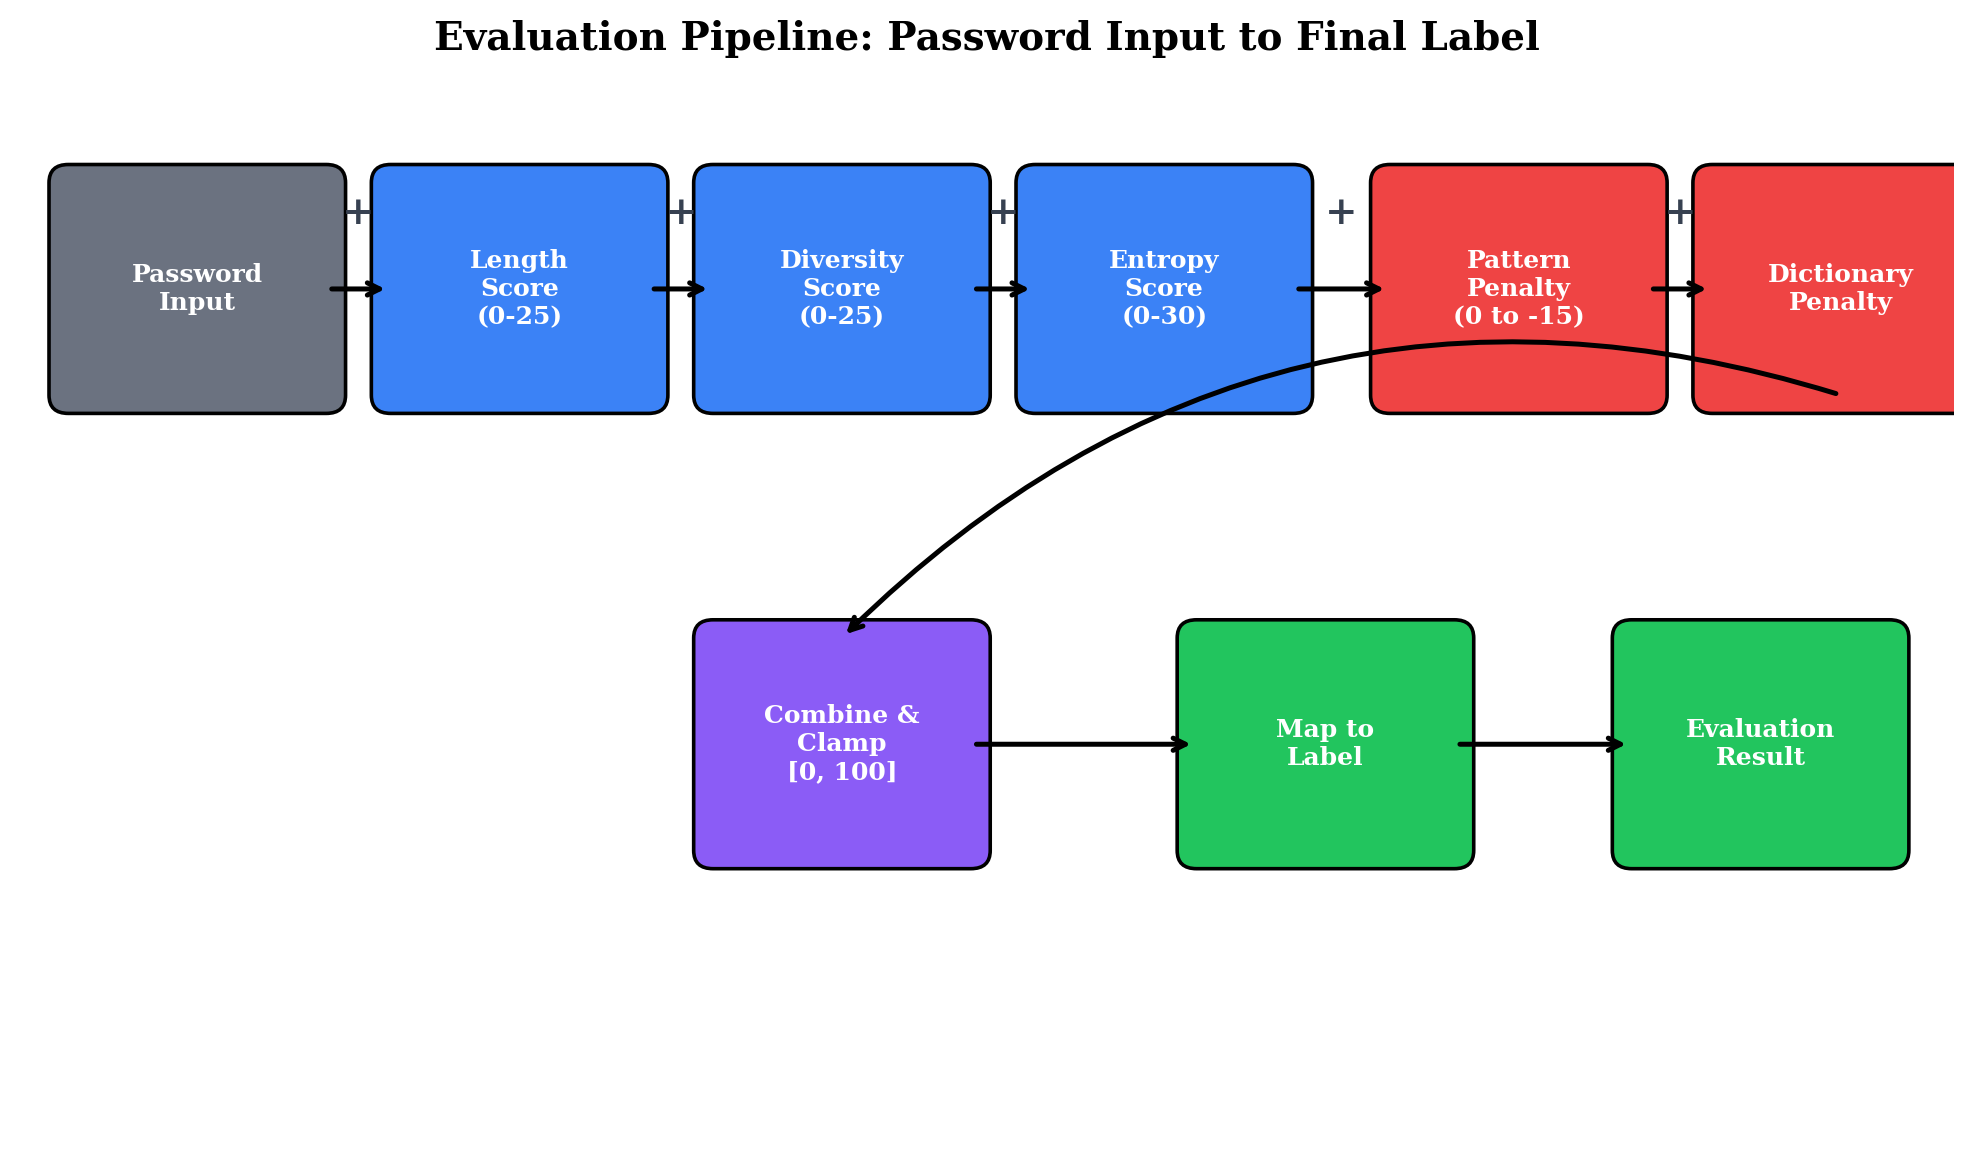
\includegraphics[width=0.85\textwidth]{figures/evaluation_pipeline_flowchart.png}
    \caption{Evaluation pipeline: password input through five scoring dimensions to final label.}
    \label{fig:eval_pipeline}
\end{figure}

Each stage produces an intermediate result that contributes to the final score. The stages are ordered such that the positive scoring dimensions (length, diversity, entropy) are computed first, followed by the negative penalty dimensions (patterns, dictionary). This ordering ensures that the penalty calculation can reference the intermediate positive scores if needed, and that the exact-common-password cap is applied as the final step.

\subsection{Worked Example}

To illustrate how the evaluation pipeline operates, consider the password \texttt{TestPass123!}. Table~\ref{tab:worked_example} shows the step-by-step calculation.

\begin{table}[H]
\centering
\caption{Step-by-step evaluation of the password \texttt{TestPass123!}.}
\label{tab:worked_example}
\begin{tabularx}{\textwidth}{lcr}
\toprule
\textbf{Stage} & \textbf{Analysis} & \textbf{Score} \\
\midrule
1. Length & 11 characters ($\geq 8$, $< 12$) & $+15$ \\
2. Diversity & Lowercase + Uppercase + Digits + Special = 4 categories & $+25$ \\
3. Entropy & $H = 11 \times \log_2 94 \approx 72.1$ bits $\Rightarrow$ tier $\geq 60$ & $+30$ \\
4. Pattern penalty & Sequential detected (\texttt{123}) & $-5$ \\
5. Dictionary penalty & Contains \texttt{pass} and \texttt{pass123} (common passwords) & $-15$ \\
\midrule
\textbf{Raw score} & $15 + 25 + 30 + (-5) + (-15)$ & $50$ \\
\textbf{Final score} & Clamped to $[0, 100]$ & $50$ \\
\textbf{Label} & $26 \leq 50 \leq 50$ & Weak \\
\bottomrule
\end{tabularx}
\end{table}

\noindent \textit{Note:} The actual tool produces a score of 50 for this password. The entropy calculation uses a dynamic character-set size ($N = 94$ for all four categories present), yielding $H = 11 \times \log_2 94 \approx 72.1$ bits (30 entropy points). The dictionary penalty of $-15$ is applied because the password contains common-password substrings (\texttt{pass} and \texttt{pass123}), reducing the raw score from 65 to 50.

\subsection{EvaluationResult Dataclass}

The evaluation function returns an immutable \texttt{EvaluationResult} dataclass containing eleven fields: the numeric \texttt{score} (0--100), the qualitative \texttt{label} (one of four strength categories), a list of \texttt{details} (analysis observations with visual indicators for positive and negative findings), a list of \texttt{suggestions} (actionable improvement recommendations), the computed \texttt{entropy\_bits} (floating-point), the estimated \texttt{crack\_time} (a human-readable string such as ``centuries+'' or ``2 hours''), and five integer breakdown fields (\texttt{length\_pts}, \texttt{diversity\_pts}, \texttt{entropy\_pts}, \texttt{pattern\_pts}, \texttt{dict\_pts}) that store the point contribution of each scoring dimension.

The suggestions are generated within the evaluator module itself---not in the GUI---to ensure a single source of truth. Each suggestion explains both \textit{what} to change and \textit{why}, using clear, non-technical language. For example, instead of merely stating ``Add special characters,'' the suggestion reads: ``Add special characters like ! @ \# \$ \% to increase unpredictability.''

\subsection{FIFO Cache}

A manual FIFO (First-In, First-Out) cache with a maximum capacity of 32 entries stores previously computed \texttt{EvaluationResult} objects, keyed by the password string. When a password is submitted for evaluation, the cache is checked first. If a cached result exists, it is returned immediately without recomputation. When the cache exceeds its capacity, the oldest inserted entry is evicted. This mechanism is particularly effective during interactive use, where users frequently add or remove one character at a time, causing the same password prefix to be evaluated multiple times.

\clearpage

\section{Core Analysis Modules}

\subsection{Entropy Module}

The entropy module provides four public functions: \texttt{classify\_characters()}, \texttt{calculate\_entropy()}, \texttt{entropy\_score()}, and \texttt{estimate\_crack\_time()}.

\texttt{classify\_characters()} is a shared utility used by both the entropy module and the diversity scoring function in the evaluator. It uses four pre-compiled regular expressions to determine which of the four character categories (lowercase, uppercase, digits, special characters) appear in the password, returning a dictionary of boolean values. The use of pre-compiled regexes avoids the overhead of recompiling the same patterns on every call.

\texttt{calculate\_entropy()} implements the Shannon entropy formula:

\begin{equation}
H = L \times \log_2 N
\end{equation}

where $L$ is the password length and $N$ is the effective character set size, determined dynamically by which character categories are present (lowercase: $+26$, uppercase: $+26$, digits: $+10$, special: $+32$). For an 8-character lowercase-only password, this yields:

\begin{equation}
H = 8 \times \log_2 26 \approx 8 \times 4.700 \approx 37.6 \text{ bits}
\end{equation}

\texttt{entropy\_score()} maps the entropy bits to a 0--30 point score using four tiered thresholds: below 28 bits yields 5 points, 28--35 bits yields 10, 36--59 bits yields 20, and 60 bits or more yields the maximum 30 points. These thresholds were chosen to reflect the practical security implications of different entropy levels: passwords below 28 bits can be cracked in seconds, while those above 60 bits resist brute-force attacks for years or longer.

\texttt{estimate\_crack\_time()} computes the estimated time to crack the password by brute-force, assuming an attacker capable of 10 billion guesses per second (consistent with modern GPU-based cracking rigs). The total number of possible combinations is $2^{H}$, and the estimated time in seconds is $2^{H} / 10^{10}$. The function converts this value to a human-readable string using progressively larger time units (seconds, minutes, hours, days, years, thousand years, million years, billion years, centuries+). Table~\ref{tab:crack_time_tiers} shows the crack time tiers.

\begin{table}[H]
\centering
\caption{Brute-force crack time tiers (assuming $10^{10}$ guesses/second).}
\label{tab:crack_time_tiers}
\begin{tabularx}{\textwidth}{cc>{\raggedright\arraybackslash}p{5cm}}
\toprule
\textbf{Entropy Range} & \textbf{Crack Time Tier} & \textbf{Example} \\
\midrule
$< 28$ bits & Less than a second & \texttt{abc} \\
$28$--$35$ bits & Seconds to minutes & \texttt{abcdef} \\
$36$--$45$ bits & Hours to days & \texttt{TestPass1} \\
$46$--$55$ bits & Days to years & \texttt{TestPass123!} \\
$56$--$65$ bits & Years to thousand years & \texttt{aB1!xY9\#mK3} \\
$66$--$75$ bits & Thousand to million years & 16-char mixed password \\
$76$--$85$ bits & Million to billion years & 16-char all-categories password \\
$> 85$ bits & Billion years to centuries+ & 20-char all-categories password \\
\bottomrule
\end{tabularx}
\end{table}

\begin{figure}[H]
    \centering
    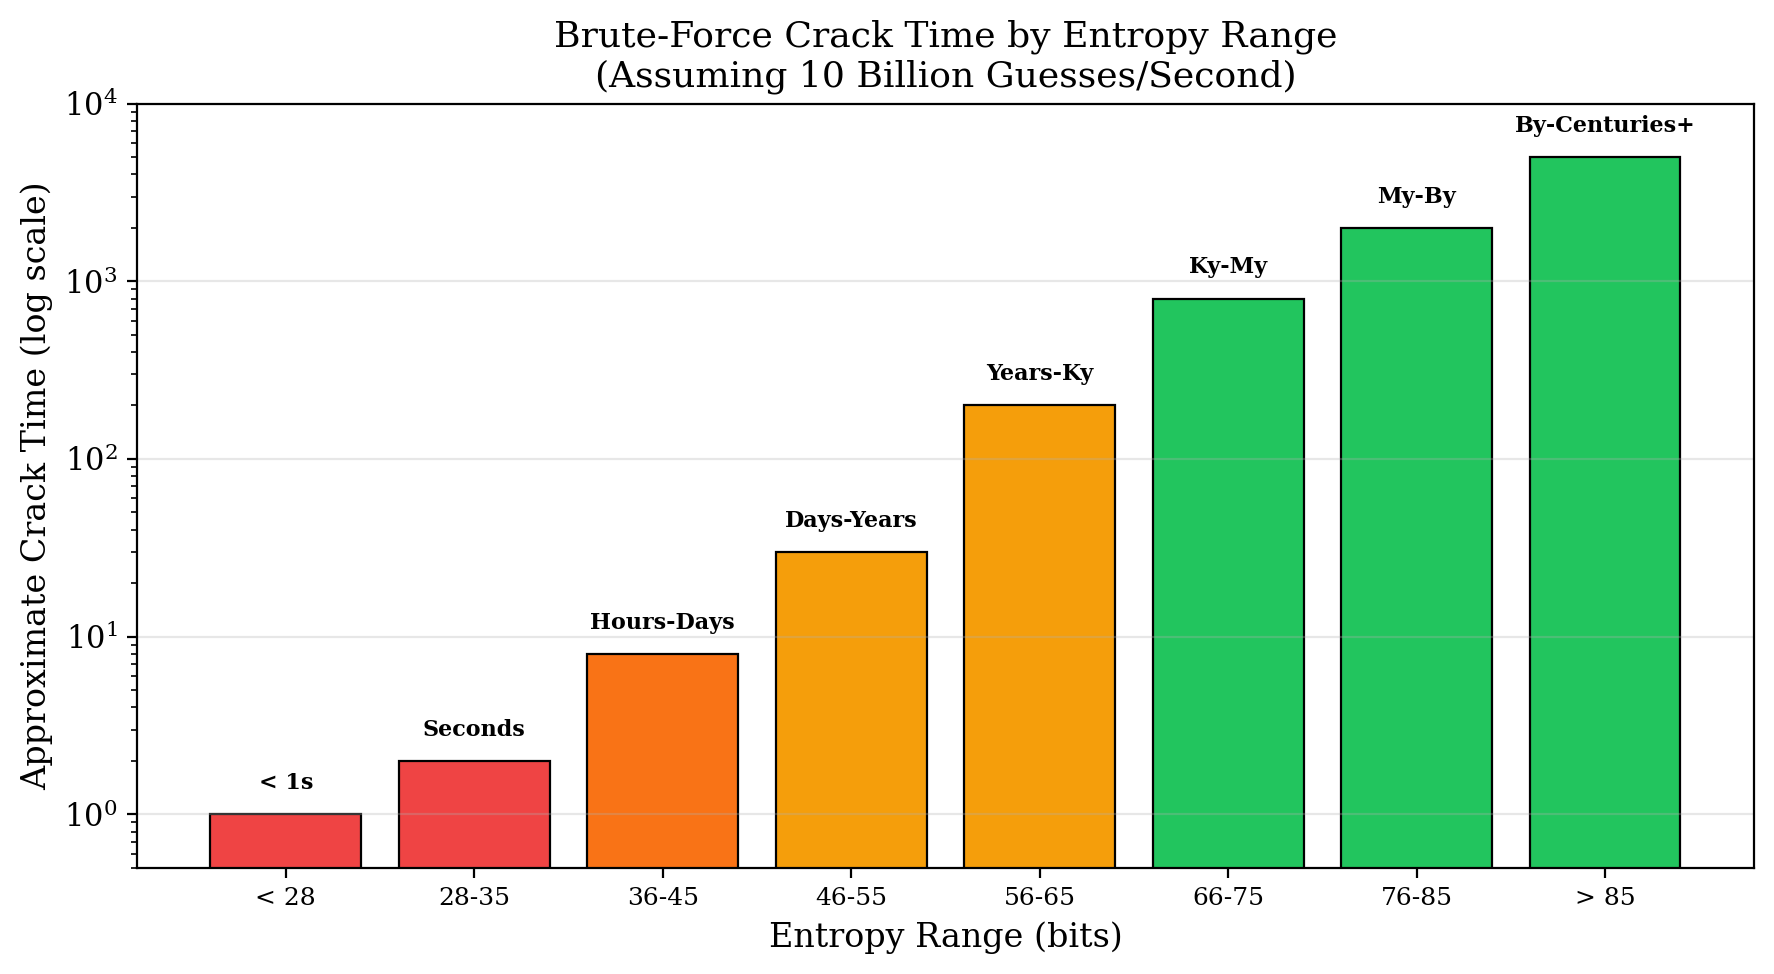
\includegraphics[width=0.85\textwidth]{figures/crack_time_tiers.png}
    \caption{Brute-force crack time by entropy range (logarithmic scale, assuming $10^{10}$ guesses/second).}
    \label{fig:crack_time_tiers}
\end{figure}

\subsection{Pattern Detection Module}

The pattern detection module provides three independent detection functions, an aggregation function, and a penalty calculation function.

\texttt{detect\_sequential()} identifies runs of three or more consecutive characters with ascending or descending ASCII code points. A critical design decision is the filtering of the input to only ASCII alphanumerics before checking for sequences. This is necessary because Unicode characters that appear in many natural-language texts (accented letters, Cyrillic characters, CJK characters) have code points that are numerically adjacent but semantically unrelated. Without this filter, legitimate passwords containing Unicode characters would trigger false-positive sequential detections. The function tracks two running counters---one for ascending sequences and one for descending---and resets the appropriate counter whenever the difference between adjacent characters is not exactly $+1$ or $-1$.

\texttt{detect\_repeated()} identifies runs of three or more identical consecutive characters (e.g., \texttt{aaa}, \texttt{111}). The implementation uses a simple running counter that increments when the current character matches the previous one and resets otherwise.

\texttt{detect\_keyboard\_patterns()} checks whether the password (converted to lowercase) contains any substring from a list of 20 known keyboard-row patterns. The patterns include the three main horizontal rows on a standard QWERTY keyboard (\texttt{qwerty}, \texttt{asdfgh}, \texttt{zxcvbn}), the QWERTZ variant (\texttt{qwertz}), numeric sequences (\texttt{1234567890} and substrings thereof), descending numeric sequences (\texttt{09876}, \texttt{98765}, \texttt{5432}), and diagonal patterns (\texttt{qazwsx}, \texttt{wsxedc}).

A distinctive feature of this implementation is the automatic generation of reversed keyboard patterns. For each pattern in the forward list, the reversed string is generated programmatically and added to the combined pattern list. For example, \texttt{qwerty} produces the reversed pattern \texttt{ytrewq}, and \texttt{asdfgh} produces \texttt{hgfdsa}. This means that passwords like \texttt{ytrewq}---which some users might believe to be less predictable than \texttt{qwerty}---are correctly identified as keyboard patterns. Table~\ref{tab:keyboard_patterns} shows a sample of the patterns and their reversed variants.

\begin{table}[H]
\centering
\caption{Sample keyboard patterns and their auto-generated reversed variants.}
\label{tab:keyboard_patterns}
\begin{tabularx}{0.7\textwidth}{lc}
\toprule
\textbf{Forward Pattern} & \textbf{Reversed Variant} \\
\midrule
\texttt{qwerty}  & \texttt{ytrewq} \\
\texttt{qwertz}  & \texttt{ztrewq} \\
\texttt{asdfgh}  & \texttt{hgfdsa} \\
\texttt{zxcvbn}  & \texttt{nbvcxz} \\
\texttt{qazwsx}  & \texttt{xswzaq} \\
\texttt{wsxedc}  & \texttt{cdexsw} \\
\bottomrule
\end{tabularx}
\end{table}

The auto-generation approach has two advantages over manually listing reversed patterns: it eliminates the risk of human error in transcribing reversals, and it automatically stays consistent whenever the forward pattern list is modified. The total combined list contains 40 patterns (20 forward + 20 reversed).

\texttt{detect\_all\_patterns()} runs all three detectors and returns a dictionary summarising the results. \texttt{pattern\_penalty\_from\_result()} computes the total penalty ($0$ to $-15$) from pre-computed detection results, allowing the penalty calculation to reuse results that were already computed for feedback generation without running the detectors again.

\subsection{Dictionary Comparison Module}

The dictionary comparison module loads a list of 181 common and leaked passwords from \texttt{common\_passwords.txt} and provides three levels of checking.

The wordlist is loaded once at module import time and stored in two data structures: a list (preserving order and enabling iteration for substring and similarity checks) and a set (enabling $O(1)$ exact-match lookup). If the wordlist file is not found, the module prints a warning to standard error and returns empty results for all checks, ensuring that the tool continues to function without the dictionary component.

\texttt{is\_common\_password()} performs an exact, case-insensitive match against the set of common passwords. The use of a set data structure guarantees $O(1)$ average-case lookup time.

\texttt{contains\_dictionary\_word()} iterates through the common-passwords list and checks whether any entry of four or more characters appears as a substring within the password (case-insensitive). An optional \texttt{limit} parameter controls the maximum number of matches to report, providing an early-exit mechanism that prevents unnecessary iteration.

\texttt{levenshtein\_distance()} implements the standard dynamic-programming algorithm for computing the Levenshtein (edit) distance between two strings. The implementation is space-optimised, using only two rows of the DP table at a time (previous and current), reducing the space complexity from $O(n \times m)$ to $O(\min(n, m))$.

\texttt{is\_similar\_to\_common()} checks whether the password is within an edit distance of 2 from any common password. Two pre-filtering steps reduce the computational cost: (1) passwords longer than 20 characters are skipped entirely (returning an empty list), and (2) entries whose length differs from the password by more than the threshold are skipped before computing the full Levenshtein distance.

\clearpage

\section{Password Generation}

The \texttt{generate\_password()} function creates a cryptographically secure random password with a default length of 16 characters (minimum 12). The generation process follows three steps:

\begin{enumerate}
    \item \textbf{Guaranteed category coverage:} One character is randomly selected from each of the four required categories (lowercase letters, uppercase letters, digits, and punctuation/symbols) using \texttt{secrets.choice()}, ensuring that the generated password always contains at least one character from each category.
    \item \textbf{Random fill:} The remaining characters (up to the target length) are selected from the combined pool of all character categories using \texttt{secrets.choice()}, providing maximum entropy.
    \item \textbf{Shuffle:} The list of characters is shuffled using \texttt{secrets.SystemRandom().shuffle()}, which uses the operating system's cryptographically secure random number generator. This step ensures that the guaranteed-category characters are not always positioned at the beginning of the password.
\end{enumerate}

The security rationale for using the \texttt{secrets} module rather than the standard \texttt{random} module is that \texttt{secrets} draws from the operating system's entropy sources (e.g., \texttt{/dev/urandom} on Linux, \texttt{CryptGenRandom} on Windows), which are designed for cryptographic use. The \texttt{random} module's Mersenne Twister algorithm, while statistically adequate for simulations, is not suitable for security purposes because its internal state can be reconstructed from a sufficient number of observed outputs.

\clearpage

\section{Graphical Interface}

\subsection{Layout Design}

The application window is divided into three main areas: a header bar, an input card, and a scrollable analysis card. The body uses a \texttt{CTkScrollableFrame} to accommodate varying content heights. The analysis card uses a two-column layout, as illustrated in Figure~\ref{fig:two_column_layout}.

\begin{figure}[H]
    \centering
    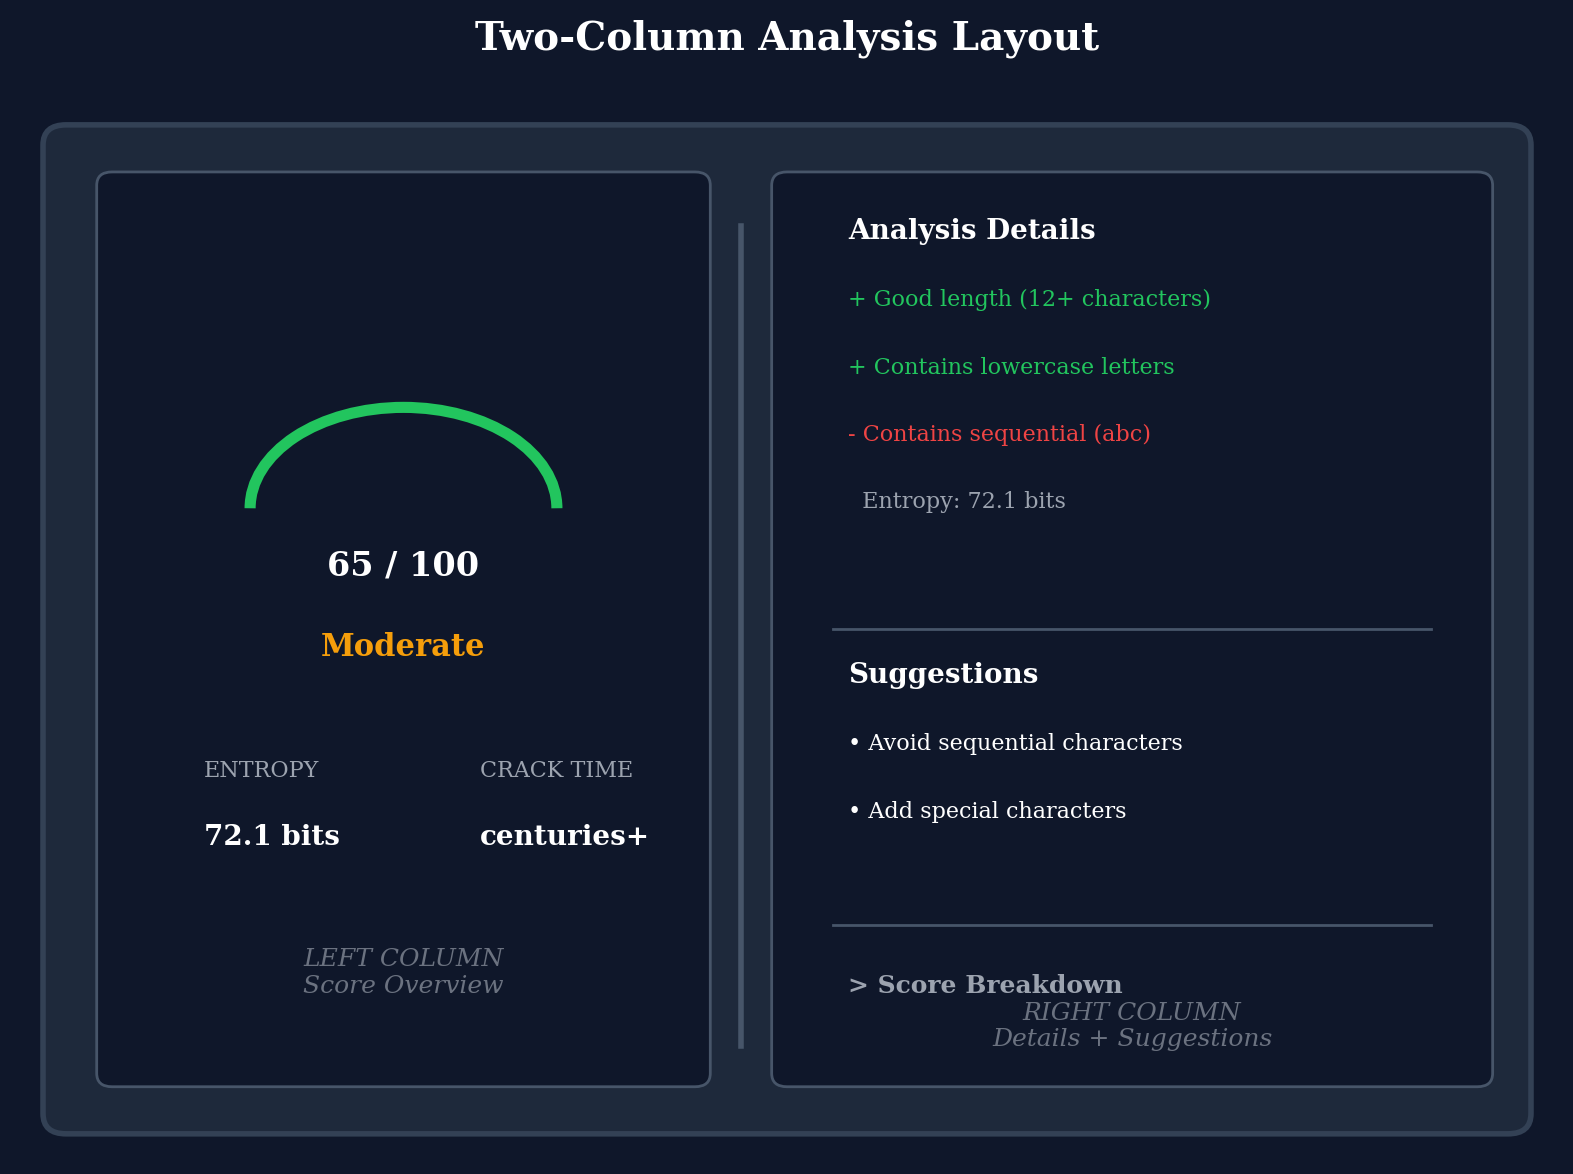
\includegraphics[width=0.85\textwidth]{figures/two_column_layout_diagram.png}
    \caption{Two-column analysis layout of the application interface.}
    \label{fig:two_column_layout}
\end{figure}

The \textbf{left column} contains the semicircular gauge (a 180-degree arc drawn on a canvas, radius 96 pixels, line width 16), the numerical score (``\textit{N} / 100''), the strength label (colour-coded text), and two information displays for entropy (bits) and estimated crack time.

The \textbf{right column} contains the analysis details section (a list of observations, each prefixed with a checkmark or cross symbol and colour-coded green or red) and the suggestions section (a list of improvement recommendations, each prefixed with a bullet point), separated by a horizontal divider.

The two-column layout was chosen over a single-column stacked layout for several reasons: it eliminates the need for scrolling within the analysis card, it allows users to see the overall score and the detailed analysis simultaneously, and it makes efficient use of the available horizontal space in a wide window.

\subsection{Animated Visual Indicators}

Both the semicircular gauge and the horizontal meter bar use smooth ease-out animations to transition from their current position to the target value. The animation uses a linear interpolation factor of 0.15 (15\% of the remaining distance per frame) with a frame interval of 16\,ms (approximately 60\,fps). This creates a smooth deceleration effect: the indicator moves quickly when the difference is large and slows down as it approaches the target value. The animation terminates when the difference between the current and target values falls below 0.5, at which point the indicator snaps to the exact target value.

The gauge is drawn as a 180-degree arc on a canvas widget. The background arc (showing the full semicircle) is drawn in a muted colour, and the filled arc (representing the current score) is drawn in the colour corresponding to the strength label. The horizontal meter bar follows the same animation logic, using a filled rectangle whose width is proportional to the score.

\subsection{Input Handling}

The password entry field is implemented as a \texttt{CTkEntry} widget with a height of 48 pixels (preventing text clipping on high-DPI displays). Input events are captured through a \texttt{KeyRelease} binding, which triggers the debounce mechanism: a 300\,ms timer is started on each keystroke, and if another keystroke occurs before the timer expires, the timer is reset. When the timer finally expires (indicating that the user has paused typing), the evaluation function is called automatically.

The visibility toggle button switches the entry field between masked mode (showing bullet characters) and plaintext mode. The toggle uses Unicode symbols for cross-platform compatibility: a hollow circle when the password is hidden and a filled circle when the password is visible.

The ``Generate Strong Password'' button fills the entry field with a newly generated password, automatically toggles the visibility to ``shown,'' and immediately triggers the evaluation, so the user can see the strength assessment of the generated password without any additional action.

\subsection{Window Configuration}

The application window is configured with a fixed size of 1000$\times$780 pixels, set as non-resizable, and centred on the screen. The fixed size ensures that the two-column layout is always displayed correctly without the need for responsive adjustments. The window uses the dark primary background colour (\texttt{\#0f172a}) and a consistent 8-pixel-base spacing system throughout the interface.

\subsection{Colour System}

Four strength colours are applied consistently across all visual indicators:

\begin{itemize}
    \item \textbf{Red} (\texttt{\#ef4444}): Very Weak
    \item \textbf{Orange} (\texttt{\#f97316}): Weak
    \item \textbf{Yellow} (\texttt{\#f59e0b}): Moderate
    \item \textbf{Green} (\texttt{\#22c55e}): Strong
\end{itemize}

These colours are applied to the gauge arc, the meter bar fill, the strength label text, and the score label, providing redundant visual encoding of the password strength assessment.

\begin{figure}[H]
    \centering
    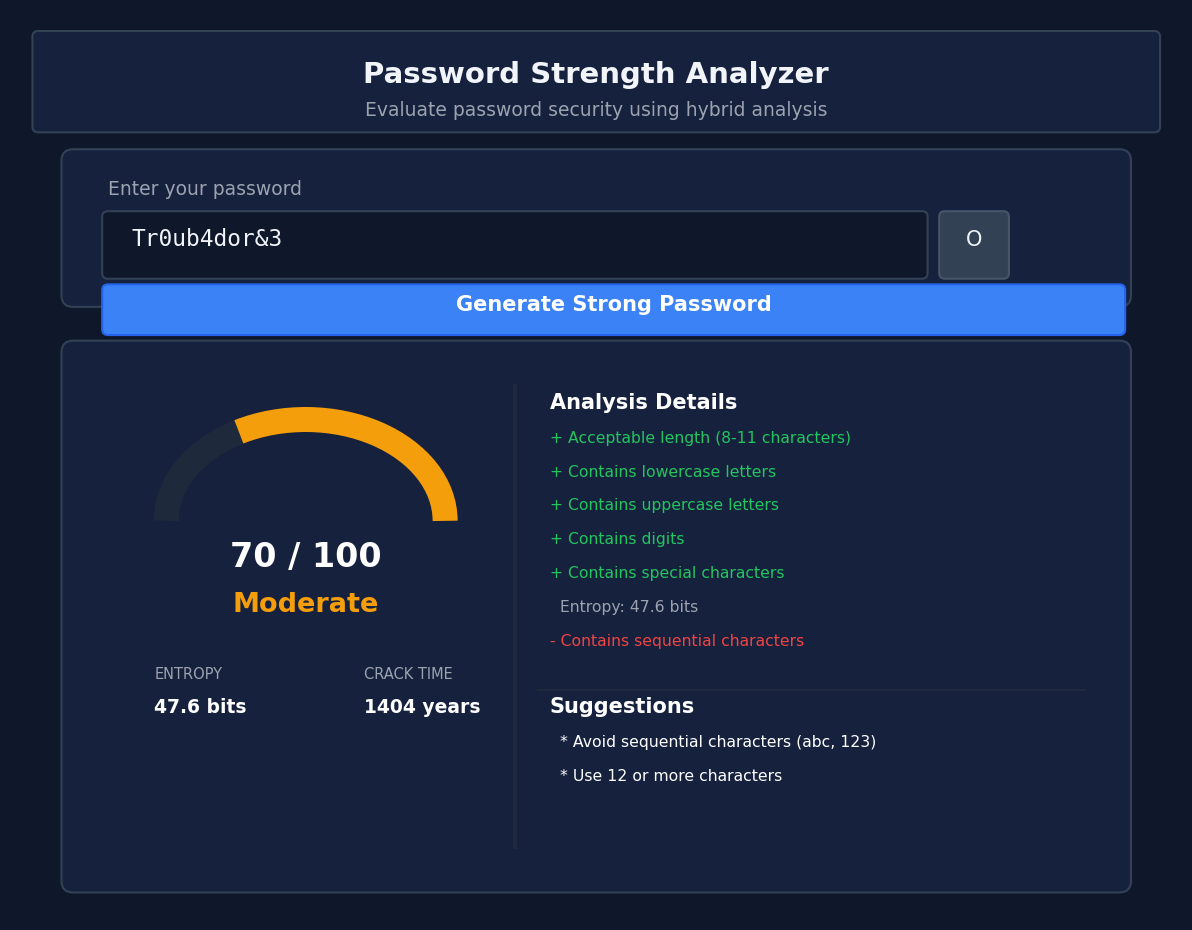
\includegraphics[width=0.85\textwidth]{figures/ui_screenshot_main.png}
    \caption{Screenshot of the Password Strength Analyzer evaluating a sample password.}
    \label{fig:ui_screenshot}
\end{figure}

\subsection{Design Decisions}

Several design decisions merit explanation:

\begin{itemize}
    \item \textbf{Why no Analyze button:} The 300\,ms debounce provides real-time feedback that is faster and more natural than requiring the user to click a button after each modification. The analysis is triggered automatically and the results update continuously, reducing the number of steps required to evaluate a password.

    \item \textbf{Why named scoring constants:} All scoring parameters are defined as named constants rather than ``magic numbers'' embedded in the code. This makes the scoring model transparent---anyone reading the evaluator module can immediately see the weights and thresholds---and makes it easy to tune the model by changing only the constant definitions.

    \item \textbf{Why suggestions live in the evaluator:} Improvement suggestions are generated within the evaluator module, not in the GUI, to ensure a single source of truth. If the evaluation logic changes (e.g., a new penalty is added), the corresponding suggestions are automatically included in the evaluation result without requiring any GUI changes.

    \item \textbf{Why two columns:} A single-column stacked layout would require scrolling to see both the overall score and the detailed analysis. The two-column layout presents all information above the fold, allowing users to see the full assessment at a glance.
\end{itemize}

\subsection{Score Breakdown Visualization}

A distinctive feature of the graphical interface is the toggleable ``Score Breakdown'' panel, which provides a visual decomposition of the final score into its five constituent dimensions. The panel displays five labelled horizontal bars---one for each scoring dimension (Length, Diversity, Entropy, Pattern, Dictionary)---with the bar length proportional to the point contribution and the colour indicating whether the contribution is positive (green) or negative (red).

The breakdown is hidden by default, showing only a ``Score Breakdown'' toggle button with a right-pointing arrow (\texttt{$\triangleright$}). When clicked, the panel expands to reveal the five bars, and the arrow changes to a downward-pointing arrow (\texttt{$\triangledown$}). Clicking again collapses the panel. This design was chosen for several reasons:

\begin{itemize}
    \item \textbf{Progressive disclosure:} Casual users who only want a quick strength assessment are not overwhelmed with detailed scoring information. Advanced users, educators, and security students can expand the breakdown to understand exactly how each dimension contributed to the final score. This follows the principle of progressive disclosure, which recommends showing the most essential information first and making detailed information available on demand.

    \item \textbf{Transparency as a feature:} No mainstream online password checker provides a per-dimension score breakdown. Most checkers present only a qualitative label (``Weak,'' ``Strong'') or a numerical score without explaining how it was computed. The breakdown panel directly supports the tool's core design philosophy of transparency and explainability---users can see not only \textit{that} their password scored 50/100, but \textit{why}: Length +15, Diversity +25, Entropy +30, Pattern $-5$, Dictionary $-15$.

    \item \textbf{Educational value:} The breakdown makes the relative weight of each scoring dimension immediately visible. A user can see, for example, that increasing their password's length from 8 to 12 characters would add 7 points (from 15 to 22 in the length dimension), while adding a special character would add 6 points (from 18 to 24 in the diversity dimension). This makes the scoring model tangible and actionable.

    \item \textbf{Implementation:} The breakdown data is stored in the \texttt{EvaluationResult} dataclass as five separate integer fields (\texttt{length\_pts}, \texttt{diversity\_pts}, \texttt{entropy\_pts}, \texttt{pattern\_pts}, \texttt{dict\_pts}), populated by the evaluation engine during scoring. The GUI reads these fields and renders the bars. This ensures that the breakdown is always consistent with the computed score, since both are derived from the same data source.
\end{itemize}

\begin{figure}[H]
    \centering
    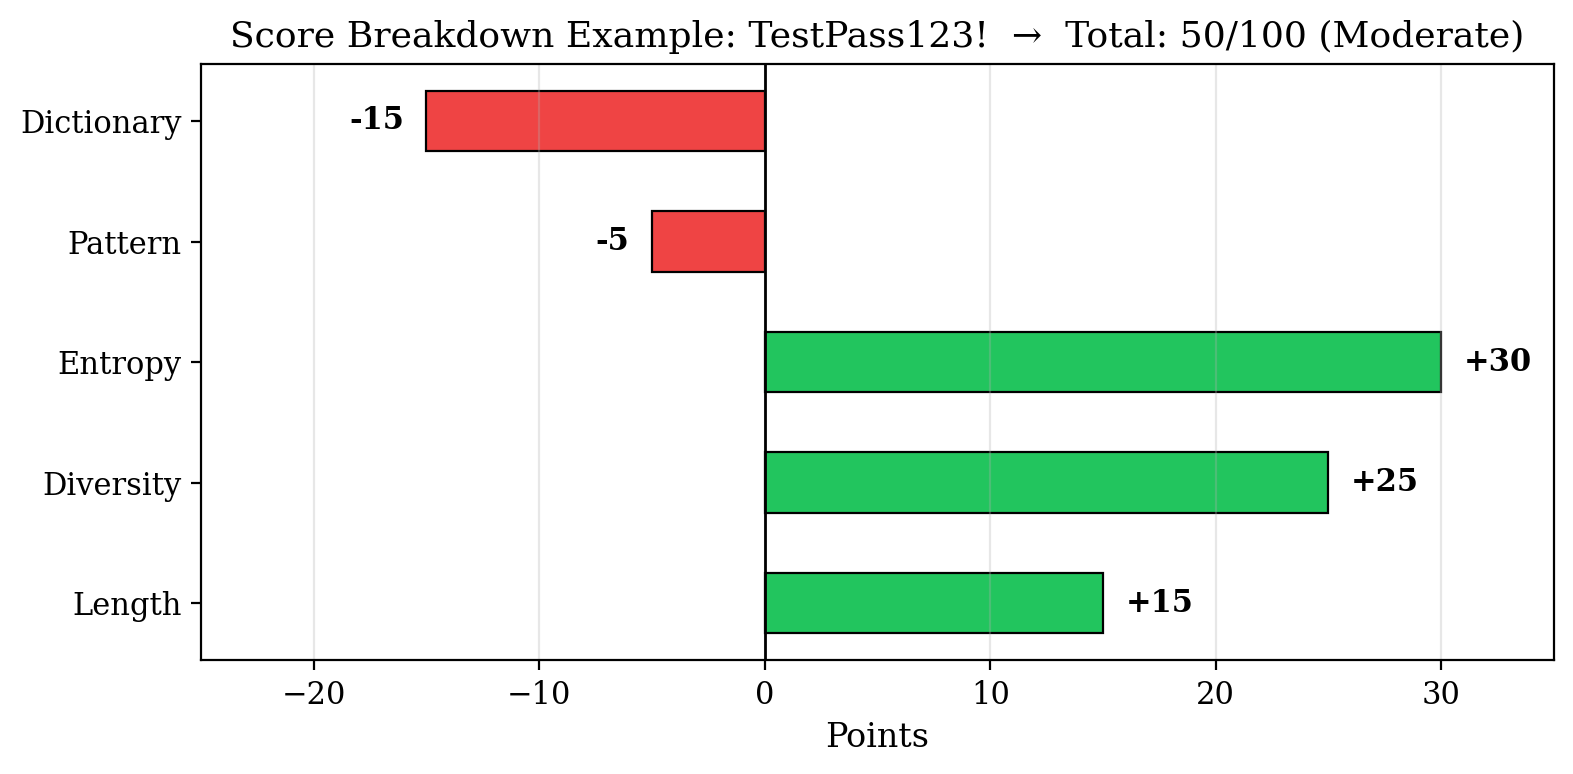
\includegraphics[width=0.85\textwidth]{figures/score_breakdown_example.png}
    \caption{Example score breakdown for the password \texttt{TestPass123!}, showing the point contribution of each dimension.}
    \label{fig:score_breakdown_example}
\end{figure}


\section{Summary}

This chapter described the implementation of the password strength evaluation tool in detail. The evaluation engine processes passwords through a five-stage pipeline, combining length scoring, character diversity assessment, entropy estimation, pattern detection, and dictionary comparison into a single transparent 0--100 score. The three core analysis modules (entropy, patterns, and dictionary check) each implement specific detection and scoring logic, with particular attention to the automatic generation of reversed keyboard patterns and the use of Levenshtein distance for similarity checking. The graphical interface provides real-time feedback through an animated dark-themed dashboard with a two-column layout. The next chapter presents the testing methodology and evaluation results.